\section{`Discrete PSYCHE'}
\label{sec:pureshift__dpsyche}

The last pure shift method in this chapter is completely original, and represents perhaps the most fruitful attempt so far at optimising pure shift experiments.
It relies on what is essentially a `temporal discretisation' of the PSYCHE waveform and gradient combination: instead of applying a shaped pulse and a gradient simultaneously, hard pulses and gradients are interleaved in the PSE (\cref{fig:dpsyche_pulseq}).

\begin{figure}[htb]
    \centering
    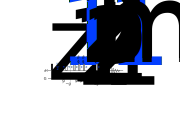
\includegraphics[draft=false]{pp/pureshift/dpsyche.png}
    \caption[dPSYCHE pulse sequence]{
        dPSYCHE pulse sequence.
        Gradient amplitudes are $(g_1, g_2) = (35\%, 41\%)$; the gradients in the PSE $g_2$ are applied with a duration of \SI{500}{\us}.
        The hard pulses in the PSE are applied with an RF amplitude of \SI{18}{\kHz}.
        The delay $\tau$ is set to $1/(4 \cdot T_\text{chunk})$, and allows for J-coupling to be refocused in the middle of the chunk.
    }
    \label{fig:dpsyche_pulseq}
\end{figure}

For this reason I have dubbed this experiment the `discrete PSYCHE', or dPSYCHE for short.
There are two major reasons why this is more amenable towards optimisation than many of the previous experiments:
\begin{enumerate}
    \item Pulses and gradients are no longer applied simultaneously, which makes simulation of the experiment \textit{extremely} fast compared to the original PSYCHE.
        This opens up the possibility of entirely theoretical optimisations, as the noise can be completely eliminated from the cost function.
        
    \item There are much fewer `pulse points' than in the original PSYCHE: effectively, the phase and flip angle of every hard pulse has to be optimised, leading to $2m$ parameters.
        Even for $m \sim 10$, this is quite tractable if the optimisation is noiseless.
\end{enumerate}

One downside of this is that it is difficult, or perhaps even impossible, to explain how the PSE works.%
\footnote{Of course, we could simulate it and say that it works because the maths says it does; but that isn't very illuminating. The optimisations done in this thesis are somewhat like a scaled-down version of machine learning, in that they produce better results at the cost of interpretability.}
For a symmetric PSE where $\beta_1 = \beta_m$ (and so on) it is probably possible to reuse an explanation based on PSYCHE-style CTP selection, but this is clearly inapplicable if the flip angles and phases are scrambled.

\subsection{Speeding up dPSYCHE simulations}
\label{subsec:pureshift__dpsyche_simulations}

To begin, I first explain how the exact simulation of dPSYCHE experiments can be greatly accelerated through efficient propagator calculations.
Although Spinach\autocite{Hogben2011JMR} is the leading simulation package for NMR, and covers an extremely impressive range of experiments, this generality also prevents it from providing optimal performance for any single experiment.
As it turns out, handwritten, specialised Matlab code can outperform Spinach by orders of magnitude.

The NMR simulations developed here simply use the density operator formalism in Hilbert space, as outlined in \cref{sec:theory__density_operators}.
The Zeeman basis is used, and non-unitary transformations such as relaxation are neglected.
Propagation under the Liouville--von Neumann equation (\cref{eq:lvn_interaction_integrated}) requires the calculation of matrix exponentials $\exp(-\mi H\tau)$.
For an $N \times N$ matrix, the matrix exponential requires $O(N^3)$ time to calculate (and for a system containing $p$ spins, we have $N = 2^p$); it is often this which is the bottleneck in NMR simulations.
Minimising the number of matrix exponentials, and/or their computational cost, is the key to achieving speedups, as will be shown in the following text.%
\footnote{Note that in my simulations, I simply used the builtin \texttt{expm} Matlab function, which implements the matrix exponential using a combination of the scaling-and-squaring method and Pad\'e approximation\autocite{Higham2005SIAMJMAA}.
This is in contrast to Spinach, which primarily uses a scaled-and-squared Taylor series (according to the \texttt{propagator.m} file, various other methods supposedly did not `live up to their marketing').
An in-depth discussion of matrix exponential methods is outside the scope of this thesis, but can be found in a classic paper by Moler and Van Loan\autocite{Moler2003SIAMR}.}

Generally, the accurate simulation of pulsed field gradients requires the sample to be divided up into $n$ discrete slices, each simulated with a different $\Hgrad$.\footnote{In simple cases this can be avoided by simply removing all terms with the wrong coherence orders as we know they will be dephased (\cref{eq:generalised_rephasing_2}), but this is too naive an approach for pure shift techniques.}
Thus, a very naive implementation of the dPSYCHE experiment would require $mn$ matrix exponentials, one per pulse per slice.
The overall structure of the code would resemble \cref{lst:dpsyche_slow}.%
\footnote{Strictly speaking, there is a slight inaccuracy in this code: the final gradient should have strength \texttt{-2G} and not \texttt{G}, but that is a minor detail which I leave out for clarity in the code.}
Note that the term \texttt{H\_free}, and the corresponding propagator \texttt{U\_free}, technically refer to the interaction-picture free Hamiltonian, $\HfreeI$.

\begin{mylisting}[htb]
    \centering
\begin{tcbminted}{matlab}
% loop over slices
for slce=1:n
    H_grad = I_z * G * z(slce);

    % loop over pulse points
    for pulse_point=1:m
        H_pulse = (c_x(pulse_point) * I_x) + (c_y(pulse_point) * I_y);

        % calculate propagators; m*n total matrix exponentials
        U_pulse = expm(-1j * (H_free + H_pulse) * t_pulse);
        U_grad = expm(-1j * (H_free + H_grad) * t_grad);

        rho = U_grad * U_pulse * rho * U_pulse' * U_grad';
    end
end
\end{tcbminted}
\caption[Naive dPSYCHE code]{Rough structure of a naive dPSYCHE implementation. Note that I use the variable name \texttt{slce} as \texttt{slice} is an existing builtin Matlab function.}
\label{lst:dpsyche_slow}
\end{mylisting}

It is not difficult to come up with a more sensible approach which cuts this down by a factor of $m$: since the pulses are not applied together with the gradients, the pulse propagators $U_{\symup{pulse}}$ can be pre-calculated outside of the loop.
Furthermore, all of the gradients within the PSE are the same, so $U_{\symup{grad}}$ can be moved out of the inner loop (\cref{lst:dpsyche_fast1}).

\begin{mylisting}[htb]
    \centering
\begin{tcbminted}{matlab}
% precalculate pulse propagators; m total matrix exponentials
for pulse_point=1:m
    H_pulse = (c_x(pulse_point) * I_x) + (c_y(pulse_point) * I_y);
    U_pulse(m) = expm(-1j * (H_free + H_pulse) * t_pulse);
end

% loop over slices
for slce=1:n
    % calculate gradient propagators; n total matrix exponentials
    H_grad = I_z * G * z(slce);
    U_grad = expm(-1j * (H_free + H_grad) * t_grad);
    
    % loop over pulse points
    for point=1:m
        rho = U_pulse(m) * rho * U_pulse(m)';
        rho = U_grad * rho * U_grad';
    end
end
\end{tcbminted}
\caption[Slightly faster dPSYCHE code]{Rough structure of a slightly faster implementation of dPSYCHE.}
\label{lst:dpsyche_fast1}
\end{mylisting}

Spinach, which is designed to be general, has no idea that these optimisations are possible, so is naturally rather slower.
However, even this is relatively inefficient.
It can be shown that the two components of the gradient propagator, $\HfreeI$ and $\Hgrad$, actually commute with one another (even in the strong coupling case).
Thus, we can write:
\begin{equation}
    \label{eq:split_propagator}
    \exp[-\mi(\HfreeI + \Hgrad)\tau] = \exp(-\mi\HfreeI\tau) \exp(-\mi\Hgrad\tau)
\end{equation}
(in general, for matrices $A$ and $B$, $\exp(A + B) = \exp(A)\exp(B)$ if and only if $[A, B] = 0$).
This on its own does not reduce the number of matrix exponentials required, but notice now that $\Hgrad$ is a sum of $I_{iz}$ terms and is therefore \textit{diagonal} in the Zeeman basis.
The exponential of a diagonal matrix is almost trivial to calculate, as we only need to exponentiate the diagonal \textit{elements:}
\begin{equation}
    \label{eq:expm_diagonal}
    \exp
    \begin{pmatrix}
        \lambda_1 & 0 & \ldots & 0 \\
        0 & \lambda_2 & \ldots & 0 \\
        \vdots & \vdots & \ddots & \vdots \\
        0 & 0 & \ldots & \lambda_n \\
    \end{pmatrix}
    = 
    \begin{pmatrix}
        \exp(\lambda_1) & 0 & \ldots & 0 \\
        0 & \exp(\lambda_2) & \ldots & 0 \\
        \vdots & \vdots & \ddots & \vdots \\
        0 & 0 & \ldots & \exp(\lambda_n) \\
    \end{pmatrix}.
\end{equation}
Instead of using the $O(N^3)$ \texttt{expm(M)} function, this can instead be done in $O(N)$ time using \texttt{diag(exp(diag(M)))} (the \texttt{diag} Matlab function converts a diagonal matrix to a vector of its diagonal entries, and vice versa).
So, we now require only $m + 1$ `true' matrix exponentials.
At this point, our matrix exponentials have almost been eliminated and the largest remaining bottleneck is almost certainly the matrix \textit{multiplications} required for the propagation.
We can cut these down by a factor of two simply by calculating the overall propagator
\begin{equation}
    \label{eq:overall_propagator}
    U_{\symup{total}} = U_n\cdots U_2U_1
\end{equation}
and then performing the propagation only at the very end:
\begin{equation}
    \label{eq:overall_propagation}
    \rho = U_{\symup{total}} \rho_0 \adj{U_{\symup{total}}}
\end{equation}
instead of performing every individual step $\rho \to U_1\rho_0\adj{U_1}$.
The final optimised code therefore resembles that in \cref{lst:dpsyche_fast2}.

\begin{mylisting}[htb]
    \centering
\begin{tcbminted}{matlab}
% precalculate propagator due to free evolution during gradient
% only 1 matrix exponential
U_free = expm(-1i * H_free * t_grad);

% precalculate pulse propagators; m total matrix exponentials
for pulse_point=1:m
    H_pulse = (c_x(pulse_point) * I_x) + (c_y(pulse_point) * I_y)
    U_pulse(m) = expm(-1j * (H_free + H_pulse) * t_pulse)
end

% loop over slices
for slce=1:n
    % initialise propagator for this slice
    U_slce = eye(2 ^ p);

    % calculate gradient propagators; no matrix exponentials required
    H_grad = I_z * G * z(slce);
    U_grad = U_free * diag(exp(diag(-1j * H_grad * t_grad)));

    % loop over pulse points
    for point=1:m
        U_slce = U_pulse(m) * U_slce;
        U_slce = U_grad * U_slce;
    end

    % perform propagation only at the end
    rho = U_slce * rho * U_slce';
end
\end{tcbminted}
\caption[Fast dPSYCHE code]{Rough structure of a fast dPSYCHE implementation.}
\label{lst:dpsyche_fast2}
\end{mylisting}

The performance of this handwritten code as compared to Spinach is summarised in \cref{tbl:dpsyche_simulations}.
In all cases, the spectra produced by the two methods were entirely equivalent.
It should be noted that the handwritten code does not even utilise CPU parallelisation, whereas Spinach does.
I investigated the possibility of parallelising the loop over slices (replacing the outer \texttt{for} in \cref{lst:dpsyche_fast2} with \texttt{parfor}): however, this in fact made the code \textit{slower}, presumably due to overhead.
This is a good thing: it means that \texttt{parfor} can be used in an external loop, e.g.\ for the parallel simulation of the dPSYCHE experiment on different spin systems.

\begin{table}[htb]
    % matlab_nmr_jy/research/compare_dpsyche.m
    \begin{tabular}{cccc}
        \toprule
        \textbf{Number of spins} & \textbf{Number of couplings} & \multicolumn{2}{c}{\textbf{Execution time (s)}} \\
        \cmidrule{3-4}
                                 & & Spinach & Handwritten \\
                                 \midrule
        \multirow{1}{*}{1}       & 0 & 3.33 & 0.35 \\
        \midrule
        \multirow{2}{*}{2}       & 0 & 4.59 & 0.32 \\
                                 & 1 & 6.22 & 0.32 \\
                                 \midrule
        \multirow{4}{*}{3}       & 0 & 9.90  & 0.43 \\
                                 & 1 & 12.95 & 0.45 \\
                                 & 2 & 31.86 & 0.47 \\
                                 & 3 & 35.01 & 0.48 \\
                                 \midrule
        \multirow{7}{*}{4}       & 0 & 30.59  & 1.02 \\
                                 & 1 & 38.63  & 0.99 \\
                                 & 2 & 44.61  & 1.04 \\
                                 & 3 & 365.04 & 1.52 \\
                                 & 4 & 446.03 & 1.57 \\
                                 & 5 & 521.72 & 1.57 \\
                                 & 6 & 588.31 & 1.69 \\
        \bottomrule
    \end{tabular}
    \caption[Comparison of wall-clock times for dPSYCHE simulations]{
        Comparison of wall-clock times for dPSYCHE simulations.
        The dPSYCHE sequence used contained 15 pulses, each applied with a flip angle of \ang{15} and a phase of \ang{0}.
        Spin systems were generated pseudo-randomly.
        All timings were measured on a 2019 MacBook Pro with a \qty{2.6}{\GHz} 6-core Intel i7 CPU (although CPU parallelisation was not used).
    }
    \label{tbl:dpsyche_simulations}
\end{table}

\subsection{Optimisations and experimental evaluation}
\label{subsec:pureshift__dpsyche_optimisation}

As previously discussed, the fact that the dPSYCHE experiment can be very quickly simulated opens up the potential for entirely computational optimisation of the pulse sequence.
For any arbitrary spin system, it is trivial to remove all the couplings \textit{in silico} and simulate a pulse--acquire spectrum: this gives us a theoretically perfect pure shift spectrum.
The simulated dPSYCHE experiment (on a system with couplings) can then be compared against this.
The entire process is repeated using $s$ different spin systems, and the cost function is defined as:
\begin{equation}
    \label{eq:f_diff_dpsyche}
    f_\text{diff,2} = \frac{1}{s}\sum_s \Biggl\lVert \frac{\symbf{S}_\text{re} - c\symbf{T}_\text{re}}{c\lVert \symbf{T}_\text{re} \rVert} \Biggr\rVert^2
\end{equation}
where $\symbf{S}$ is the dPSYCHE spectrum, and $\symbf{T}$ is the target spectrum.
The prefactor $c$ will be discussed later; for now I treat it as $1$.
This cost function appears superficially very similar to $f_\text{diff}$ (discussed in \cref{subsec:pureshift__optim_techniques}), and is based on the same principle that we want the spectra $\symbf{S}$ and $\symbf{T}$ to match one another, but there are several points of note:
\begin{itemize}
    \item The spectrum $\symbf{S}_\text{re}$ is not scaled down by its norm. This means that the sensitivity penalty no longer comes from the difference in the noise (as was previously the case), but rather directly from the difference in peak intensity.
        Since simulated spectra are noiseless, the original $f_\text{diff}$ would not work here.
    \item The division of the entire cost function by $\lVert\symbf{T}_\text{re}\rVert$ is not important if only one spin system is being simulated as it is simply a constant factor.
        However, if more than one spin system is being simulated, $\lVert\symbf{T}_\text{re}\rVert$ differs from system to system and this factor helps to essentially normalise the contributions from each spin system.
    \item The norm in the cost function here is squared.
        Again, this makes no difference to the optimum if only one spin system is being investigated, because $x^2$ is strictly increasing for $x > 0$.\footnote{It may affect the rate of convergence, but this is not something I tested.}
        However, for multiple spin systems it makes sense to square the norm, as the largest deviations will be penalised more greatly: this means that a pure shift spectrum which works reasonably well across a wide range of spin systems will be prioritised over one which works perfectly well for some and fails badly for others.
\end{itemize}

I began by first checking how many $t_1$ increments (i.e.\ chunks) were required in the simulation to obtain reliable cost function values.
If too few chunks are simulated, the resulting pure shift spectrum will have truncation artefacts, which are likely to mask artefacts from unwanted CTPs.
The value of $f_\text{diff,2}$ was thus tested with a wide variety of randomly chosen phases and angles, with the number of chunks set to 4, 8, and 16 (\cref{fig:dpsyche_td1_cf}).

\begin{figure}[htb]
    \centering
    \includegraphics[]{pureshift/td1_cf.png}%
    {\phantomsubcaption\label{fig:dpsyche_td1_cf_16_8}}%
    {\phantomsubcaption\label{fig:dpsyche_td1_cf_16_4}}%
    \caption[Comparison of $f_\text{diff,2}$ cost function with different numbers of chunks]{
        Comparison of $f_\text{diff,2}$ values when simulated with different numbers of chunks.
        16 chunks is assumed to be the `gold standard'.
        \textbf{(\subref*{fig:dpsyche_td1_cf_16_8})} Correlation between 16-chunk and 8-chunk cost functions.
        The `optimum' identified by both cost functions is plotted in green in the inset.
        \textbf{(\subref*{fig:dpsyche_td1_cf_16_4})} Correlation between 16-chunk and 4-chunk cost functions.
        The `optima' identified by the 16- and 4-chunk cost functions are plotted in green and red respectively in the inset.
    }
    \label{fig:dpsyche_td1_cf}
\end{figure}

The 16-chunk and 8-chunk $f_\text{diff,2}$ (\cref{fig:dpsyche_td1_cf_16_8}) do in fact line up quite well.
Notably, as the inset shows, they both agree on the `best' candidate (note that this is not necessarily anywhere near perfect, since it was randomly generated).
The 4-chunk $f_\text{diff,2}$ also has the correct overall behaviour (\cref{fig:dpsyche_td1_cf_16_4}).
However, its ranking of the `best' candidates is not very accurate: the 4-chunk cost function rates the red dot in the inset as the optimum, but that is only the 13th-best candidate when using the 16-chunk cost function.
Ultimately, I decided to use the 4-chunk cost function for `quick and dirty' optimisations, where only an approximate optimum was required.
However, for anything requiring more accuracy, the 8-chunk cost function was used.

An optimisation was then carried out with a (rather arbitrarily chosen) setting of $m = 9$, i.e.\ nine hard pulses in the PSE.
A total of $s = 20$ spin systems were used, matching the number of CPU cores on the computer used for the optimisations: these were further subdivided into four two-spin systems, eight three-spin systems, and eight four-spin systems.
The derivative-based BFGS algorithm was used to carry out the optimisation: this is a popular line search algorithm which uses an approximate Hessian to calculate the search direction at each iteration.\autocite{Kelley1999,Nocedal2006}
No lower or upper bounds were placed on the flip angles or phases: phases can obviously simply be wrapped to the region $[0, 2\pi)$, and in the simulations, the hard pulses were modelled as being instantaneous rotations, so their flip angles can also just be wrapped to $[0, 2\pi)$.
(This would not be completely valid if realistic, finite pulses were used, since changing the flip angle would also change their duration.)
This first optimisation yielded the following optimised parameters for the nine pulses:
\begin{align}
    \{\beta_i\} &= \{\ang{118.6972}, \ang{29.8400}, \ang{107.4850}, \ang{190.4788}, \notag \\
                &\qquad \ang{138.4710}, \ang{144.5939}, \ang{18.9674}, \ang{73.8900}, \ang{130.6071}\} \label{eq:dpsyche_opt_nosens_angles} \\
     \{\phi_i\} &= \{\ang{144.5641}, \ang{173.3596}, \ang{38.9878}, \ang{146.3121}, \notag \\
                &\qquad \ang{127.7346}, \ang{7.5104}, \ang{36.9805}, \ang{110.2791}, \ang{182.3894}\}. \label{eq:dpsyche_opt_nosens_phases}
\end{align}
The fact that none of the flip angles exceeded \ang{360} here provides some justification for not using bounds in the optimisation.

\begin{figure}[htb]
    % I don't have the Matlab output data any more: it was done in
    % examples/run_opt_par() and predates some of the API rework to (e.g.)
    % enforce reproducibility. The angles and pulses are just taken from the
    % TopSpin data. :/ OK not ideal, I know, but too bad. Can't change it.
    % There IS one way to retrieve the data: rewind the entire git repo to this
    % date and rerun it.
    \centering
    \includegraphics[]{pureshift/dpsyche_nosens_vs_psyche}%
    {\phantomsubcaption\label{fig:dpsyche_nosens_vs_psyche_dp}}%
    {\phantomsubcaption\label{fig:dpsyche_nosens_vs_psyche_p}}%
    \caption[Comparison of optimised dPSYCHE and PSYCHE]{
        \textbf{(\subref*{fig:dpsyche_nosens_vs_psyche_dp})} dPSYCHE experiment acquired using the flip angles and phases in \cref{eq:dpsyche_opt_nosens_angles,eq:dpsyche_opt_nosens_phases}.
        The $\beta$ hard pulses in the PSE were applied with an RF amplitude of 
        \textbf{(\subref*{fig:dpsyche_nosens_vs_psyche_p})} (Double-saltire) PSYCHE experiment acquired with $\beta = \ang{20}$.
        \datacode{6A-211027}
    }
    \label{fig:dpsyche_nosens_vs_psyche}
\end{figure}

To evaluate the quality of the decoupling on a real sample, the dPSYCHE experiment was performed experimentally, and the results compared against a PSYCHE experiment (\cref{fig:dpsyche_nosens_vs_psyche}).
Firstly, it is worth pointing out that a pure shift spectrum (even if not a very good one) was obtained: this validates the form of the PSE and the optimisation approach used here, especially considering that the optimisation was not tailored towards this particular sample.
The dPSYCHE experiment clearly has much greater sensitivity than the PSYCHE experiment; however, the decoupling quality is extremely poor.
The reason for this is likely because the optimisation is prioritising sensitivity too highly over purity, and ultimately stems from the factor $c$ in \cref{eq:f_diff_dpsyche} which we have ignored until now.
Since $c = 1$, the optimisation is essentially guiding the dPSYCHE experiment towards having \textit{exactly the same sensitivity as a pulse--acquire experiment}.

Although this might be a nice idea in principle, it is not physically sensible: no pure shift method has sensitivity which is even close to that of a pulse--acquire experiment.
It makes more sense to scale down the target spectrum by introducing a factor of $c < 1$ into the cost function (\cref{eq:f_diff_dpsyche}); the parameter $c$ therefore represents the `target sensitivity'.
By changing the parameter $c$, we can control whether the optimisation emphasises sensitivity or purity more.
(Note that this option was \textit{not} available to us in the experimental JRSE-based optimisations in \cref{sec:pureshift__optimisation}.)

A series of new optimisations were therefore run, with $c$ ranging from $0.2$ to $1$ (\cref{tbl:dpsyche_sens}).
The 4-chunk cost function was used, and the maximum number of function evaluations capped at 5000.
Each optimisation was run 10 times with a different starting seed, and the best of the 10 results chosen for further evaluation (\cref{tbl:dpsyche_sens}).
The resulting spectra (\cref{fig:dpsyche_sens}) show that adjusting $c$ has the desired effect: larger values lead to greater sensitivity and lower purity, and vice versa.

\begin{table}[htb]
    % matlab_nmr_jy/research/optim_specdiff/opt_sens.out
    \begin{tabular}{cccc}
        \toprule
        $c$ & \textbf{Flip angles} ($^\circ$) & \textbf{Phases} ($^\circ$) & $f_\text{diff,2}$ \\
        \midrule
        1 & \makecell{59.8813, 96.0748, 111.5862, \\ 118.7285, 144.701, 176.9773, \\ 29.2866, 40.0658, 63.8237} & \makecell{355.773, 81.741, 99.8752, \\ 81.6675, 337.0056, 150.7004, \\ 105.9666, 317.9979, 27.7897} & 0.0404 \\
        \midrule
        0.8 & \makecell{81.9461, 65.311, 90.3488, \\ 106.6388, 73.3462, 196.7857, \\ 51.791, 34.8188, 53.9506} & \makecell{329.8571, 60.3564, 137.3929, \\ 68.5286, 340.74, 126.29, \\ 64.4601, 145.4714, 27.3019} & 0.0321 \\
        \midrule
        0.6 & \makecell{53.1313, 82.2547, 88.6093, \\ 161.9291, 83.462, 161.3548, \\ 14.2976, 66.2199, 53.9709} & \makecell{347.2835, 59.5518, 68.072, \\ 113.5358, 34.5537, 156.191, \\ 268.7641, 302.7427, 16.29} & 0.0250 \\
        \midrule
        0.4 & \makecell{77.2998, 127.7274, 87.6663, \\ 104.6371, 99.6474, 168.8171, \\ 8.8569, 52.7865, 58.1408} & \makecell{342.2787, 47.7526, 76.4114, \\ 97.3304, 14.2178, 163.9513, \\ 94.2575, 280.0273, 16.0971} & 0.0271 \\
        \midrule
        0.2 & \makecell{120.6613, 107.6712, 84.0427, \\ 133.5377, 82.1999, 223.122, \\ 41.1617, 41.9398, 12.016} & \makecell{347.2051, 79.4503, 109.8796, \\ 83.5017, 345.4284, 133.8355, \\ 66.4118, 201.0041, 4.4419} & 0.0261 \\
        \midrule
        0.4* & \makecell{92.4395, 133.2136, 38.9704, \\ 34.9182, 56.0256, 57.4097, \\ 31.5916, 140.1088, 128.7125} & \makecell{62.036, 16.411, 319.5634, \\ 128.4443, 49.7357, 328.5103, \\ 210.6498, 44.0123, 327.4517} & 0.0108 \\
        \bottomrule
    \end{tabular}
    \caption[dPSYCHE optimisation results for different sensitivities]{
        Results of dPSYCHE optimisations for different sensitivities.
        Note that since the cost function depends on the value of $c$, the exact value of $f_\text{diff,2}$ for these optimisations cannot be compared to one another; they are only presented here for completeness.
        The final entry, labelled with an asterisk, was run with no limit on the number of function evaluations (this is discussed further in the text).
    }
    \label{tbl:dpsyche_sens}
\end{table}

\begin{figure}[htbp]
    % matlab_nmr_jy/research/optim_specdiff/opt_sens.m
    \centering
    \includegraphics[]{pureshift/dpsyche_sens.png}%
    {\phantomsubcaption\label{fig:dpsyche_sens_d1}}%
    {\phantomsubcaption\label{fig:dpsyche_sens_d0p8}}%
    {\phantomsubcaption\label{fig:dpsyche_sens_d0p6}}%
    {\phantomsubcaption\label{fig:dpsyche_sens_d0p4}}%
    {\phantomsubcaption\label{fig:dpsyche_sens_d0p2}}%
    {\phantomsubcaption\label{fig:dpsyche_sens_p}}%
    \caption[dPSYCHE optimisations with different sensitivities]{
        \textbf{(\subref*{fig:dpsyche_sens_d1})} dPSYCHE, $c = 1$.
        \textbf{(\subref*{fig:dpsyche_sens_d0p8})} dPSYCHE, $c = 0.8$.
        \textbf{(\subref*{fig:dpsyche_sens_d0p6})} dPSYCHE, $c = 0.6$.
        \textbf{(\subref*{fig:dpsyche_sens_d0p4})} dPSYCHE, $c = 0.4$.
        \textbf{(\subref*{fig:dpsyche_sens_d0p2})} dPSYCHE, $c = 0.2$.
        \textbf{(\subref*{fig:dpsyche_sens_p})} Double-saltire PSYCHE with $\beta = \ang{20}$.
        All spectra and insets are plotted to scale to allow for sensitivity comparisons.
        \datacode{6A-211231}
    }
    \label{fig:dpsyche_sens}
\end{figure}

In this spectrum of andrographolide, the \qtyrange{3.5}{5}{\ppm} region (blue inset) is an `easier' region to decouple: there are fewer couplings here and all spin systems are firmly within the weak coupling regime.
The \qtyrange{1.5}{2.8}{\ppm} region (orange inset) is `more difficult' to decouple, especially the two peaks at \qty{2.5}{\ppm}, which are mutually strongly coupled.
The dPSYCHE spectrum with $c = 0.4$ appeared to be a good compromise between purity and sensitivity: its sensitivity was higher than that of the original (\ang{20} flip angle) PSYCHE experiment.
Furthermore, it provided good decoupling in the `easier' deshielded region and somewhat acceptable performance in the shielded region, with the notable exception of the strongly coupled peaks at \qty{2.5}{\ppm}.

I therefore ran a longer optimisation using the same starting point and with no limit on the number of function evaluations, which successfully lowered the cost function value by twofold (the last entry in \cref{tbl:dpsyche_sens}).
The pure shift spectrum obtained using these optimised pulses is shown in \cref{fig:dpsyche_optsens3}.
The decoupling quality in both regions is comparable to that in the PSYCHE spectrum, again with the exception of the strongly coupled peaks at \qty{2.5}{\ppm}.

\begin{figure}[htb]
    % matlab_nmr_jy/research/optim_specdiff/opt_sens3.m
    \centering
    \includegraphics[]{pureshift/dpsyche_optsens3.png}%
    {\phantomsubcaption\label{fig:dpsyche_optsens3_d}}%
    {\phantomsubcaption\label{fig:dpsyche_optsens3_p}}%
    \caption[dPSYCHE final optimisation with $c = 0.4$]{
        \textbf{(\subref*{fig:dpsyche_optsens3_d})} Fully optimised dPSYCHE experiment with $c = 0.4$.
        \textbf{(\subref*{fig:dpsyche_optsens3_p})} Double-saltire PSYCHE with $\beta = \ang{20}$.
        \datacode{6A-211231}
    }
    \label{fig:dpsyche_optsens3}
\end{figure}

\begin{figure}[htb]
    % matlab_nmr_jy/research/optim_specdiff/opt_sens3.m but with different pulprog
    \centering
    \includegraphics[]{pureshift/tsedpsyche_optsens3.png}%
    {\phantomsubcaption\label{fig:tsedpsyche_optsens3_d}}%
    {\phantomsubcaption\label{fig:tsedpsyche_optsens3_p}}%
    \caption[TSE-dPSYCHE final optimisation with $c = 0.4$]{
        \textbf{(\subref*{fig:tsedpsyche_optsens3_d})} Fully optimised TSE-dPSYCHE experiment with $c = 0.4$.
        \textbf{(\subref*{fig:tsedpsyche_optsens3_p})} Double-saltire TSE-PSYCHE with $\beta = \ang{20}$.
        \datacode{7A-220129}
    }
    \label{fig:tsedpsyche_optsens3}
\end{figure}

To make the dPSYCHE experiment more robust towards strong coupling, a TSE version of the sequence was also written and tested (\cref{fig:tsedpsyche_optsens3}).
This did indeed improve the decoupling at \qty{2.5}{\ppm}, as expected.
However, although the TSE-dPSYCHE version still retains its \textit{overall} sensitivity advantage over TSE-PSYCHE (especially evident in the deshielded region), this is not true of every peak: the two peaks at 1.65 and \qty{1.70}{\ppm} seem to have decreased intensities in the TSE-dPSYCHE experiment.
The reason for this remains unclear.

% number of pulses (maybe can omit?)
\iffalse
I then ran several preliminary screens to decide on the number of pulses to include in the pulse sequence.
Here, the 8-chunk cost function was used.
To save time, the total number of function evaluations was capped at 600 times the number of pulses: this, together with the fact that only one optimisation per category was run, means that these results are more suggestive rather than conclusive.
(Since the BFGS algorithm is a local optimiser, and the trajectory depends quite strongly on the initial point, the optimisation should \textit{in theory} be run with several different initial points.)
There was no clear winner, but the optimisations with 9 and 15 pulses yielded the best results; since optimising 18 parameters is easier than 30, I opted to go with 9 pulses.

\begin{figure}[htb]
    \centering
    \includegraphics[]{pureshift/opt_npulses.png}%
    \caption[Comparison of cost functions attained with different numbers of pulses]{Blah}
    \label{fig:dpsyche_opt_npulses}
\end{figure}
\fi

\todo{State optimisation?}

% state optimisation

% conclusions and future work

